%%% NOTATER %%%
% Skrive om forutsetninger?
% Vi lager et headless cms.
% Visualisere prosjektet: https://github.com/acaudwell/Gource

\clearpage

\section{Analyse av opprinnelig løsning}
Målet med å analysere det nåværende nettstedet til Sirkus Media er å kartlegge eventuelle problemerområder som burde forbedres. Når utviklingen av det nye nettstedet er ferdig vil vi sammenligne de nye testresultatene med resultatene som blir presentert i dette kapittelet.
Se figur \ref{fig:analysis-current-sirkusmedia.no} for bilde av nettsiden på PC og mobil.

\begin{figure}[H]
    \begin{center}
        \subfigure[PC]{
            \label{fig:analysis-current-sirkusmedia.no-desktop}
            \frame{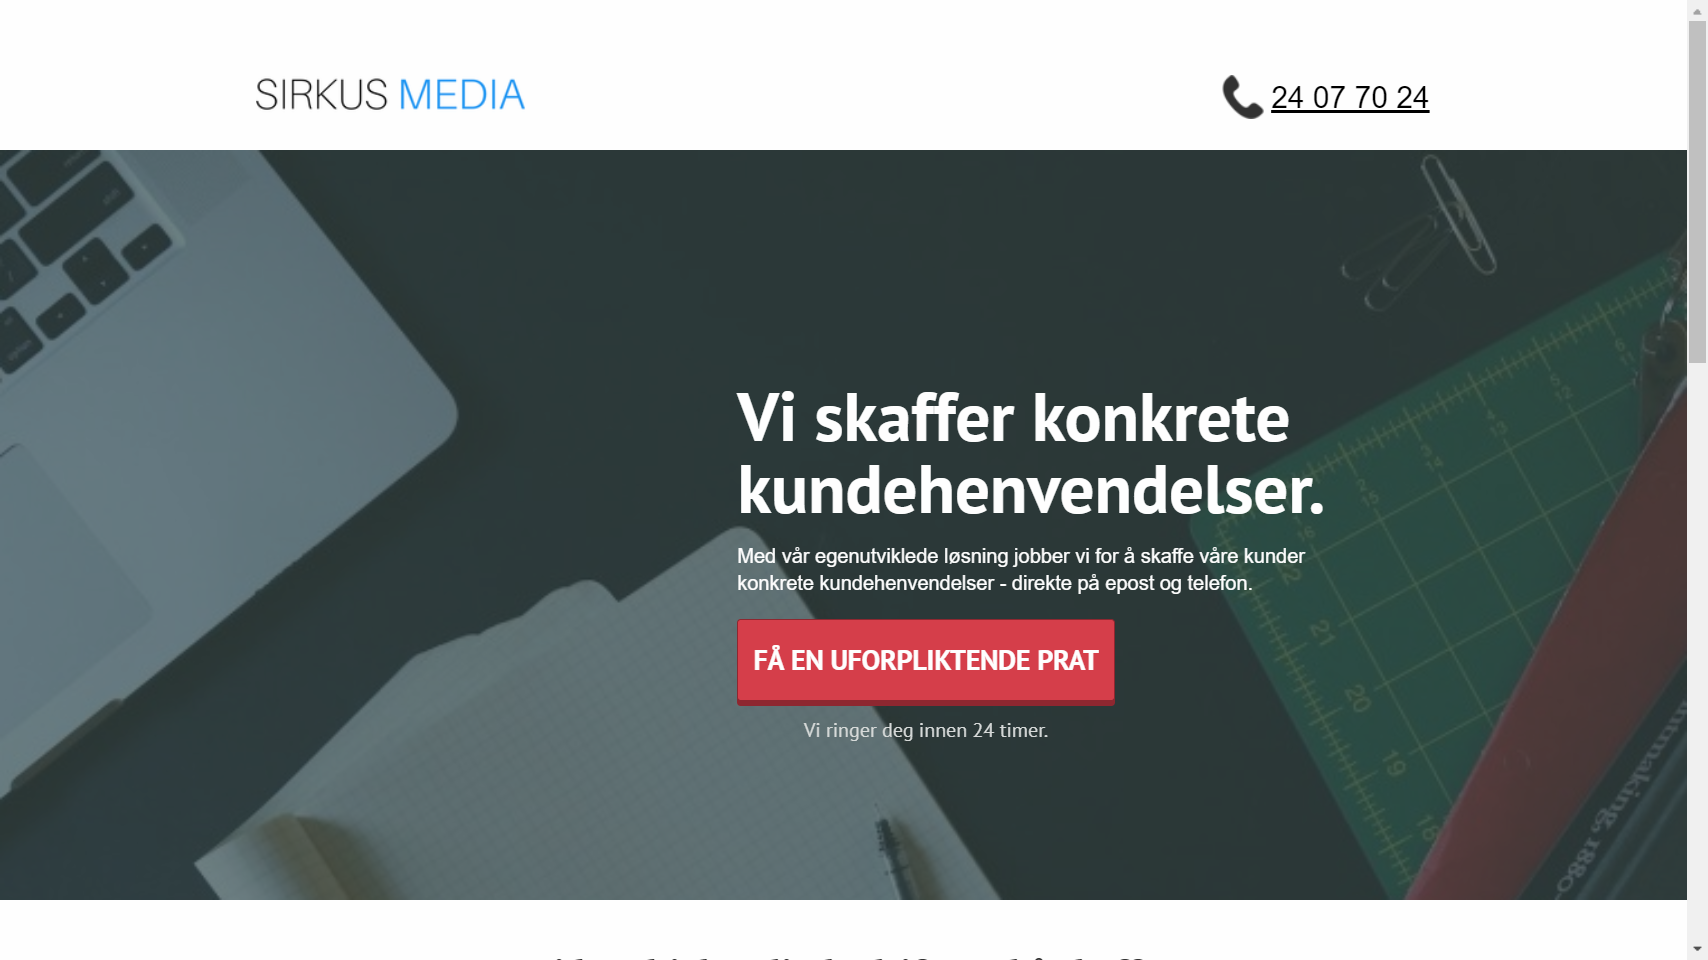
\includegraphics[width=0.7\textwidth]{bjornar/sirkusmedia_no_(1366x768).png}}
        }
        \subfigure[Mobil]{
            \label{fig:analysis-current-sirkusmedia.no-mobile}
            \frame{
\includegraphics[width=0.25\textwidth]{bjornar/sirkusmedia_no_(iPhone_6_7_8).png}}
        }
        \label{fig:analysis-current-sirkusmedia.no}
        \caption{sirkusmedia.no}
    \end{center}
\end{figure}

\subsection{Test med Google Chrome DevTools}
Google Chrome DevTools\footnote{\url{https://developers.google.com/web/tools/chrome-devtools/}} er et utviklerverktøy som følger med nettleseren Google Chrome. Det lar oss blant annet sjekke hastighet og kontrastforhold på siden og kjøre tester med Google Lighthouse.

Vi testet hastigheten til siden på det trådløse nettverket til Høgskolen i Østfold (avdeling Halden) fra en Dell XPS 13 (9350).
Resultatene måles i millisekunder.

\begin{table}[H]
\begin{tabular}{lllll}
Test & DOM & Load &  &  \\
1 & 268 & 624 &  &  \\
2 & 203 & 550 &  &  \\
3 & 216 & 560 &  &  \\
4 & 387 & 928 &  &  \\
5 & 210 & 572 &  &  \\
6 & 634 & 844 &  &  \\
7 & 309 & 857 &  &  \\
8 & 256 & 670 &  &  \\
9 & 348 & 673 &  &  \\
10 & 249 & 579 &  &  \\
\end{tabular}
\end{table}

Gjennomsnitt:\\
- DOM: 308ms\\
- Load: 614ms

Innlastningstiden til DOM beskriver hvor lang tid det tar for nettleseren å lese gjennom og analysere HTML-koden til nettsiden. Load vil si hvor lang tid det tar å laste inn DOM sammen med alle bilder, stylesheets, scripts og iframes.

\subsection{Test med Google Lighthouse}
\label{sec:analysis-current-lighthouse}

Ved å kjøre Google Lighthouse får vi resultater for hastighet, tilgjengelighet, beste praksis, søkemotoroptimalisering og progressiv webapplikasjon. Figur \ref{fig:analysis-current-lightouse-summary} viser oppsummering av resultatetene etter å ha kjørt testen. Oversikten viser at nettstedet får gode poengsummer på alle områdene. Hovedgrunnen til dette er at dagens nettsted består av kun en forside og lite informasjon. Dette begrenser muligheten for feil.

\begin{figure}[H]
    \centering
    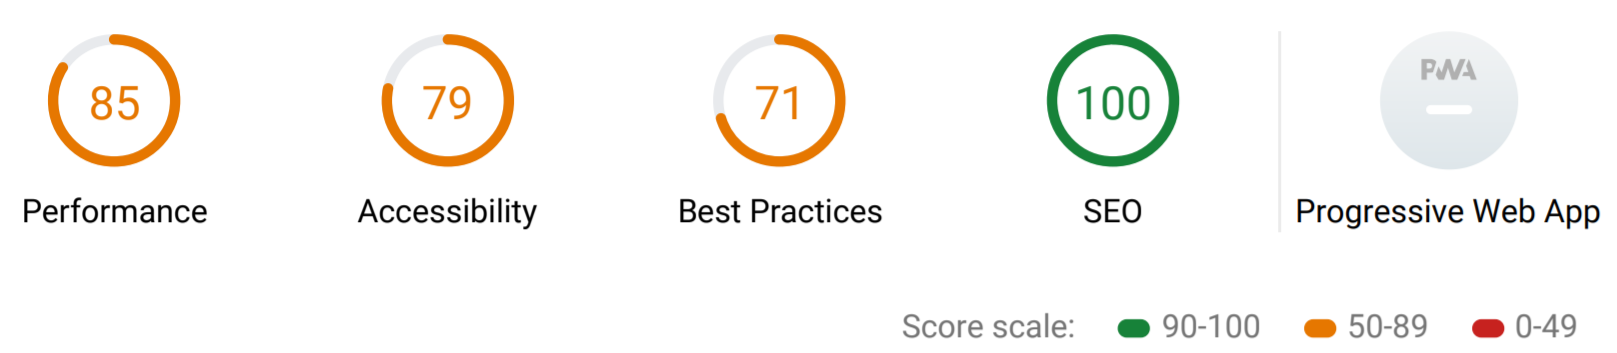
\includegraphics[width=\textwidth]{bjornar/Lighthouse-Report-mobile.png}
    \caption{Resultater fra Google Lighthouse}
    \label{fig:analysis-current-lightouse-summary}
\end{figure}

Ikonet for \q{Progressive Web App} har en feil, slik at man ikke får sett scoren. Ved hjelp av en JSON-fil\footnote{Se JSON-fil, linje 3386} som inneholder resultatene, ser man at poengscoren er på 58\%.

Denne delen av testen er egentlig ikke relevant\footnote{Sirkus Media sitt nettsted er ikke, og kommer ikke til å bli en progressiv webapplikasjon. KILDE OM PWA}, og vi vil derfor ikke se på denne, eller nevne den i andre tekniske analysener som bruker Google Lighthouse.

I rapporten kan vi se at Google laster inn nettsiden på 2,7 sekunder og at det tar 4,9 sekunder før siden blir beregnet som interaktiv. Hovedproblemet til siden er bruken av \q{render-blocking resources}\footnote{Hva er dette?}. Dette kan lett fikses og kan i følge Google spare 1,34 sekunder. Google påpeker også at det finnes 3 sikkerhetshull i JavaScript-biblioteker som blir brukt på nettsiden. Dette er ikke ønskelig, da dette øker risikoen for uønskede hendelser.

Full rapport for Google Lighthouse testen kan leses i vedlegg X.

\subsection{Checkbot}
\begin{figure}[H]
    \centering
    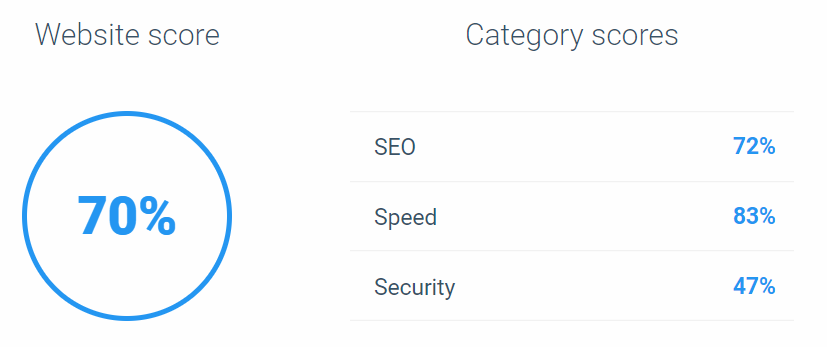
\includegraphics[width=0.75\textwidth]{bjornar/checkbotio-summary.png}
    \caption{Checkbot.io summary}
    \label{fig:analysis-current-checkbot-summary}
\end{figure}

Checkbot\footnote{https://checkbot.io} tester sikkerhet, hurtighet og søkemotoroptimalisering. Figur \ref{fig:analysis-current-checkbot-summary} viser oppsummering av resultatene. En mer detaljert rapport kan leses under vedlegg X. Denne testen viser en god poengsum når det gjelder totalt for gjennomsnittet. Isolert sett ser vi at sikkerheten til nettstedet drar ned gjennomsnittet betydlig. Den fulle rapporten viser at dette kommer av at nettsiden ikke bruker HSTS, \q{content sniffing protection}, \q{clickjack protection}, \q{XSS protection} og at det ikke skjuler server-versjon data.

\subsection{Color Contrast Analyzer}
\label{sec:analysis-current-color-contrast-analyzer}
Color Contrast Analyzer\footnote{\url{https://accessibility.oit.ncsu.edu/tools/color-contrast-chrome/}} tar bilde av nettstedet og scanner deretter kontrasten. Områder med bedre kontrast utheves og får lyse kanter. Jo mer markante kanter, desto mer kontrast.

\begin{figure}[H]
    \centering
    \makebox[\textwidth]{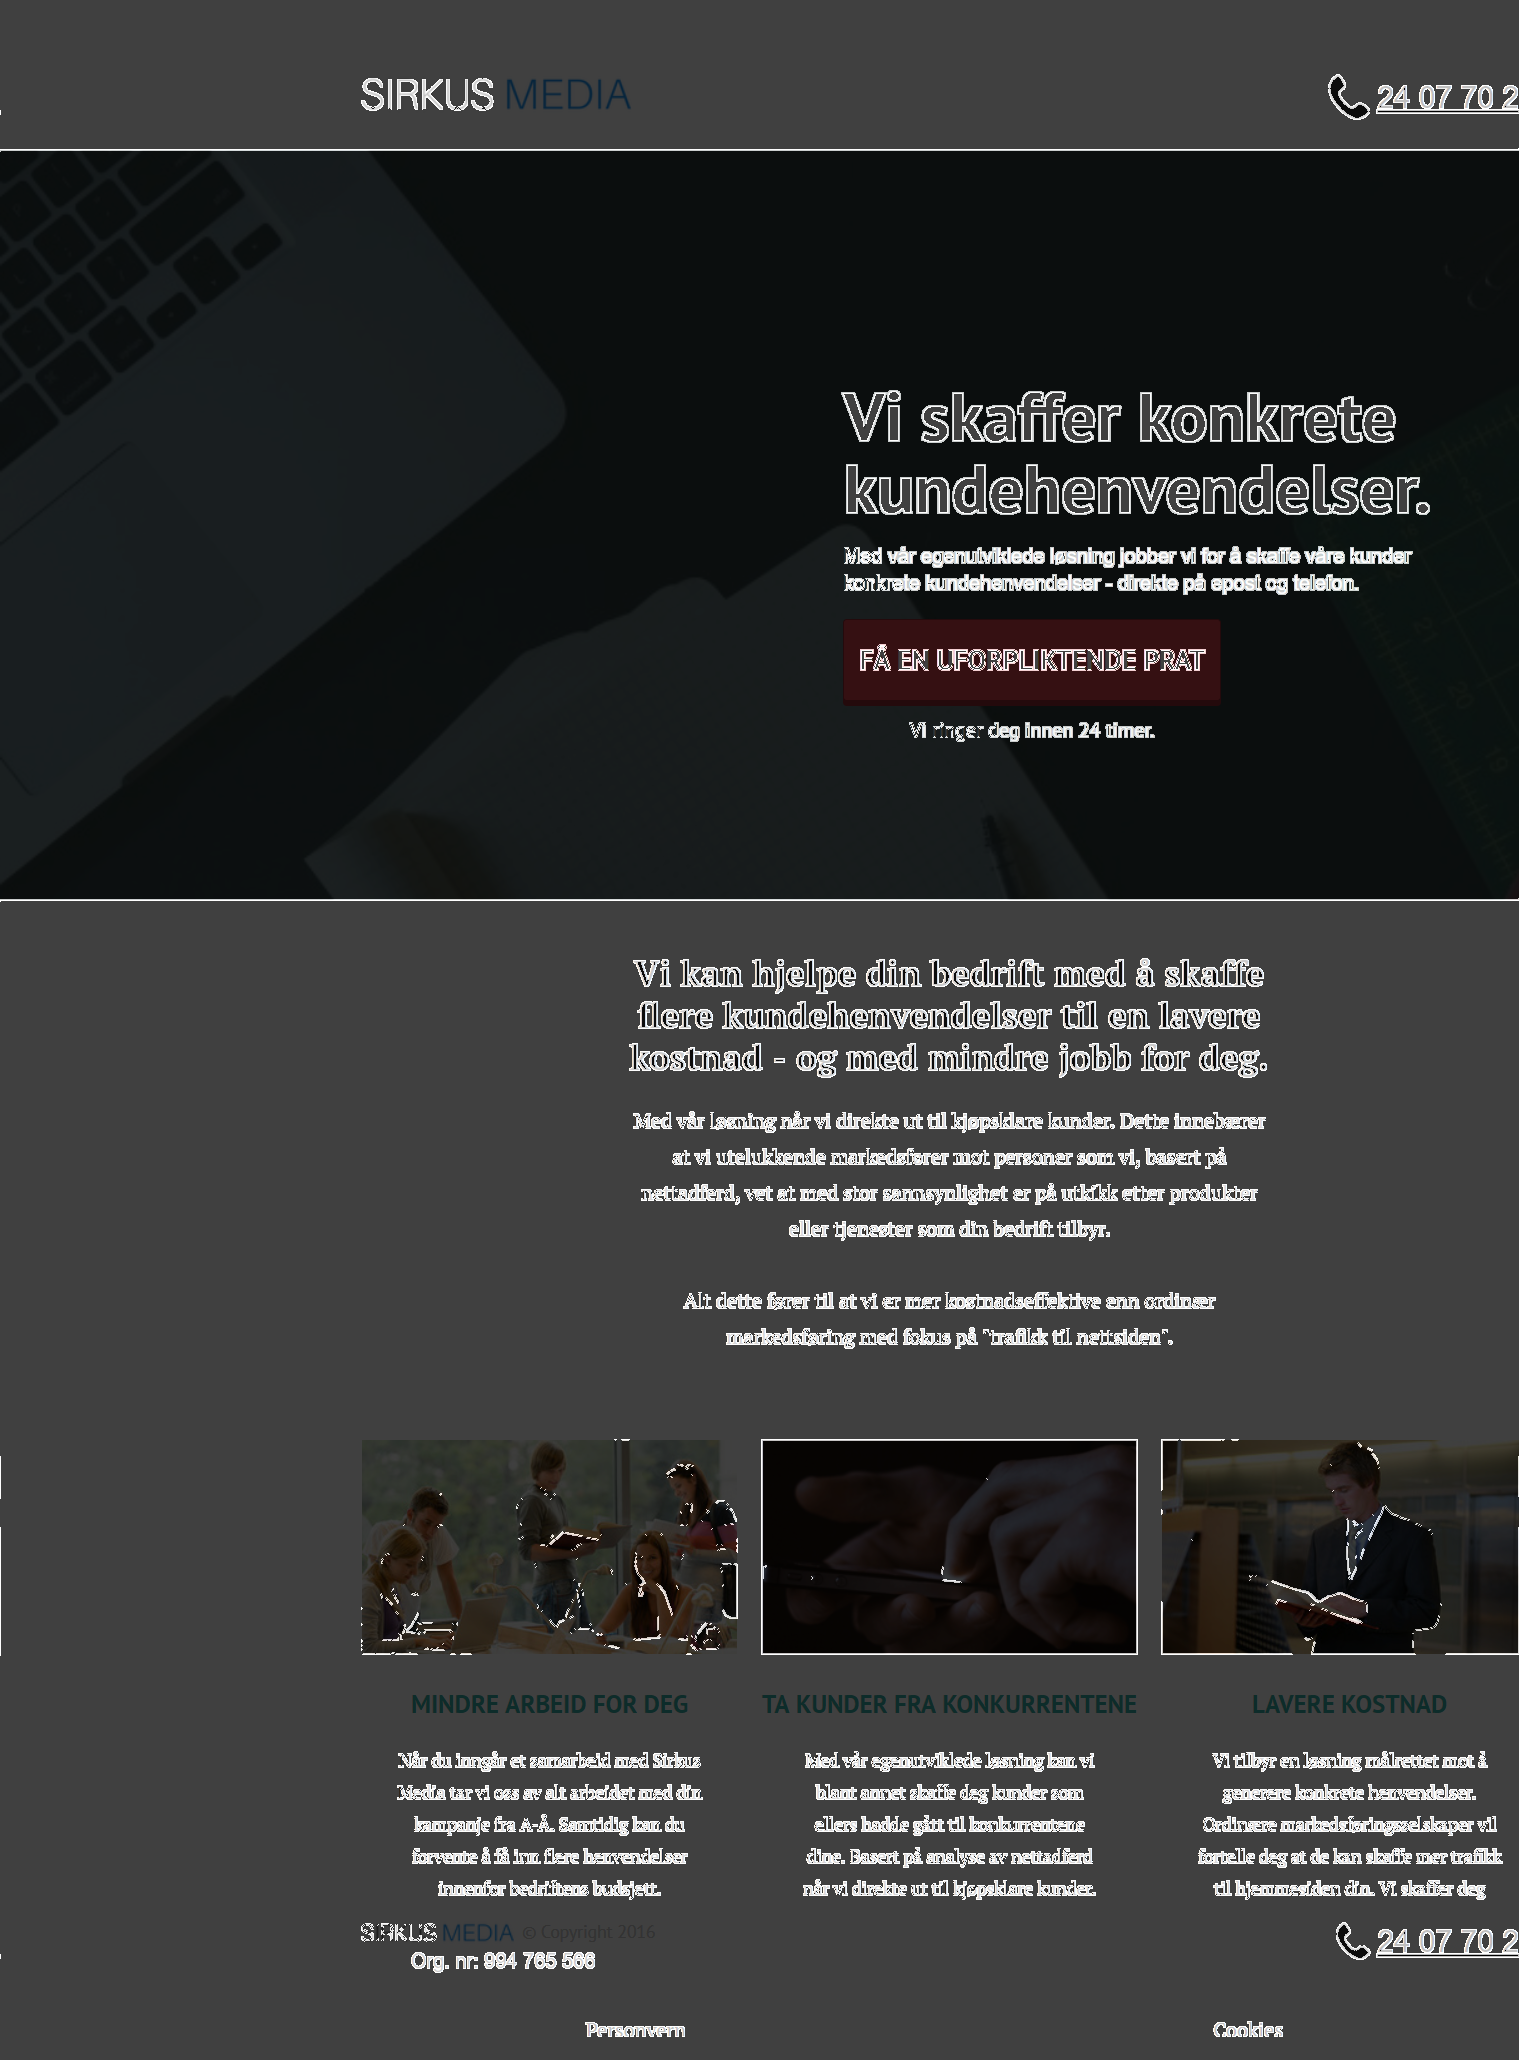
\includegraphics[width=0.80\paperwidth]{bjornar/contrast-wcag-aa-small.png}}
    \caption{CCA resultat AA}
    \label{fig:analysis-current-cca-aa}
\end{figure}

\begin{figure}[H]
    \centering
    \makebox[\textwidth]{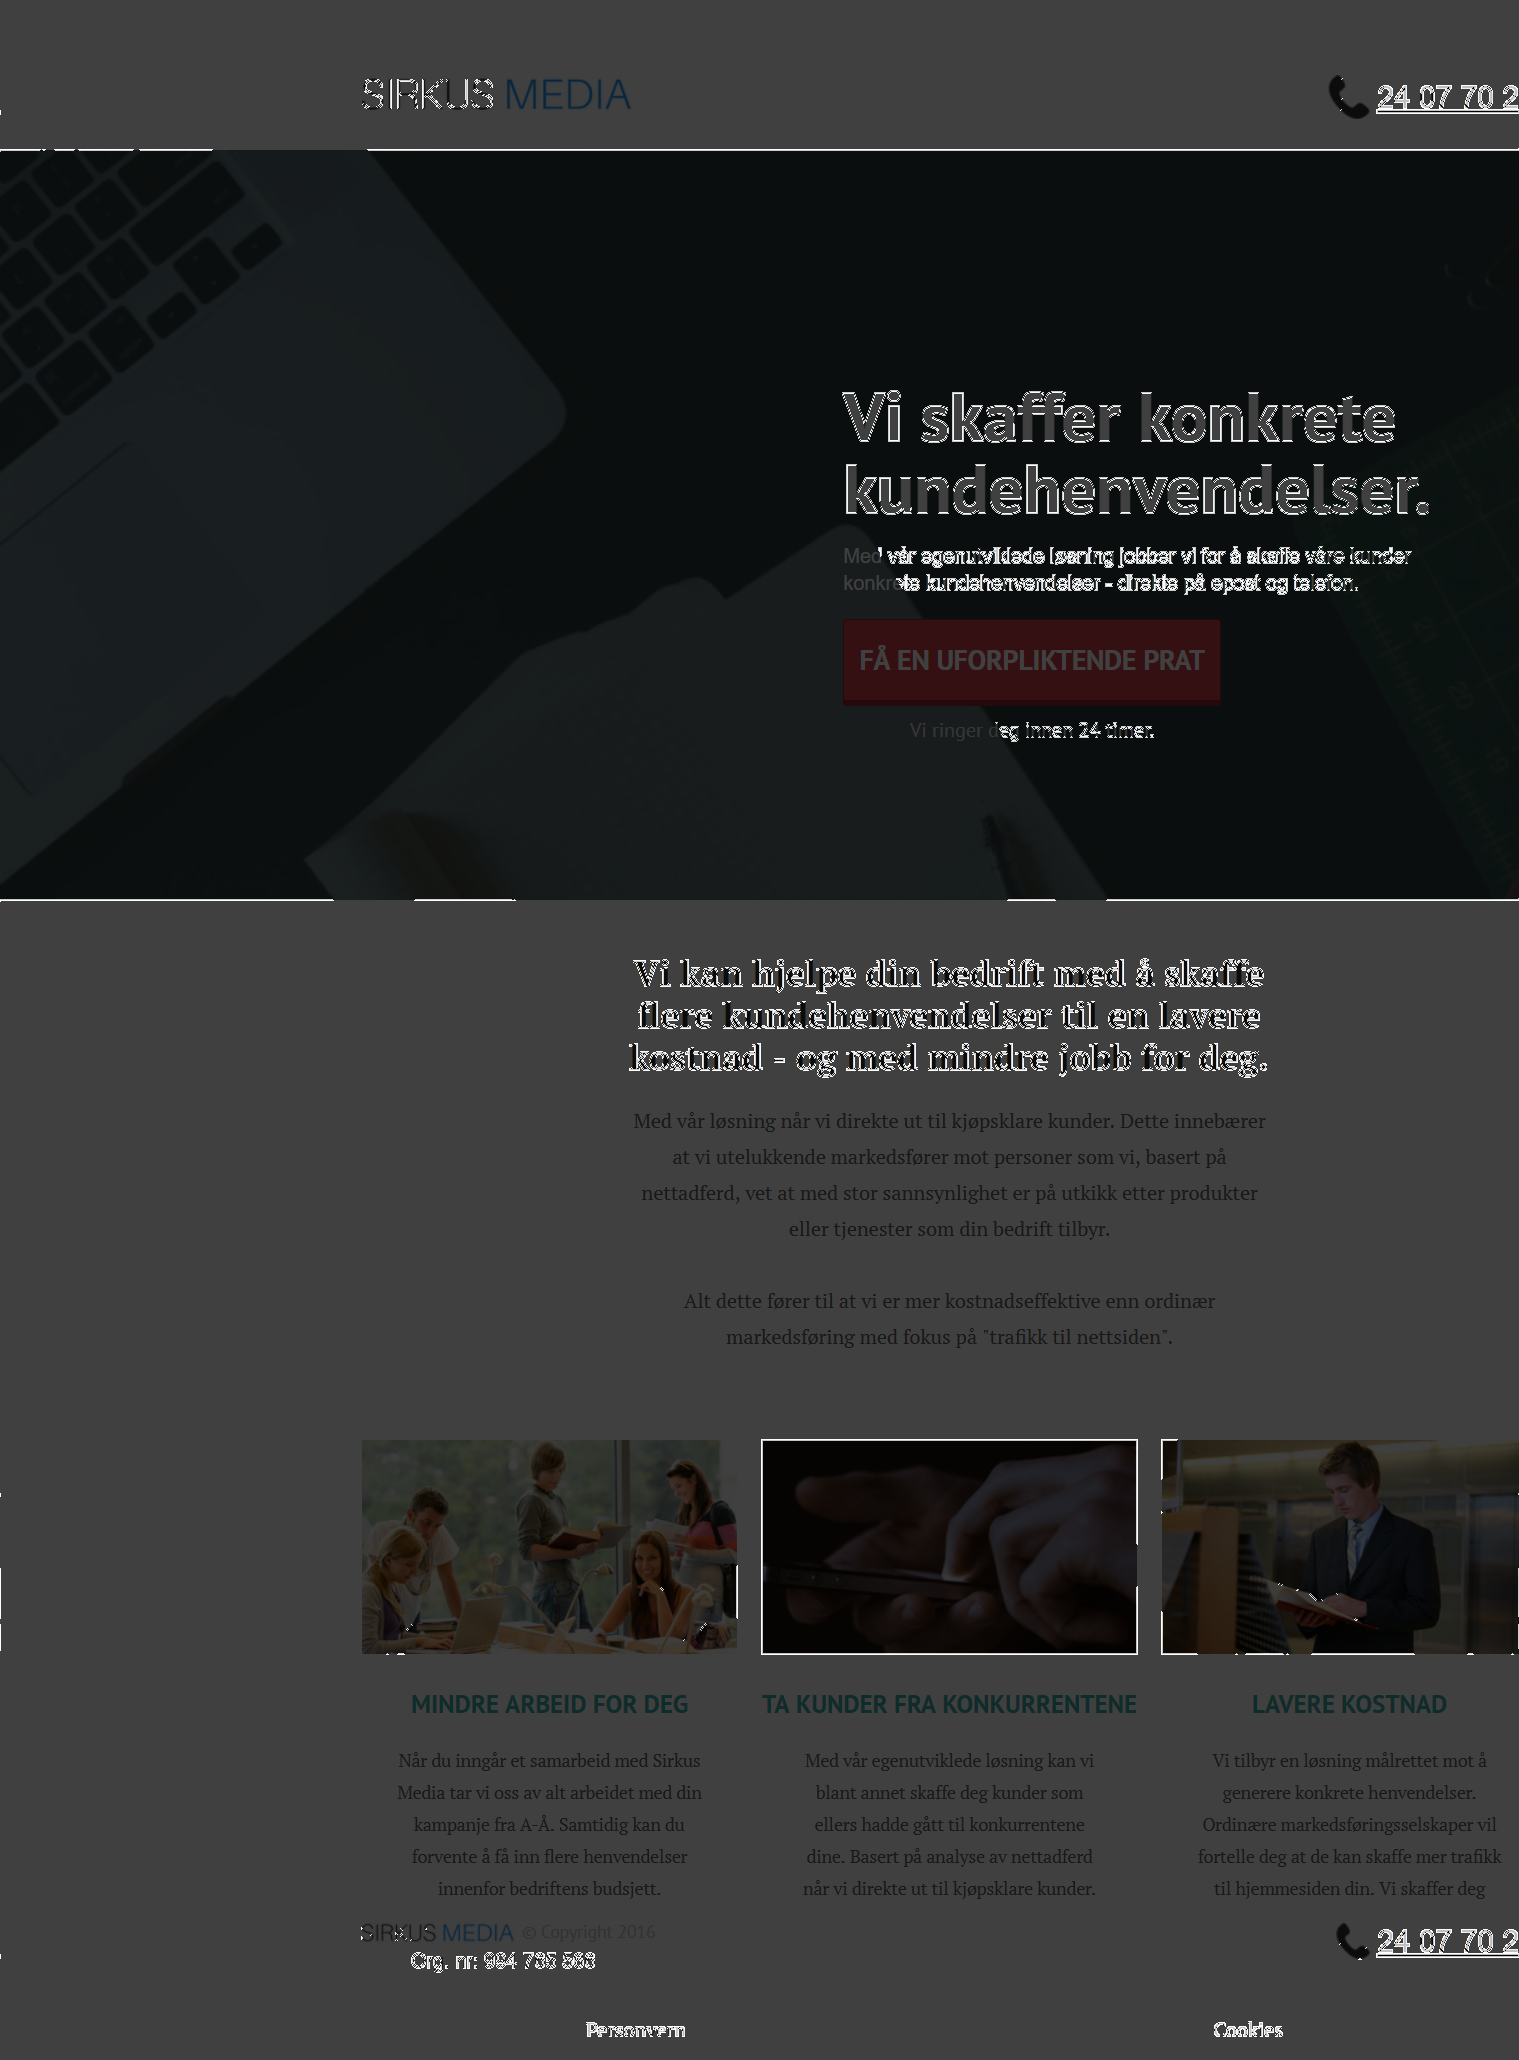
\includegraphics[width=0.80\paperwidth]{bjornar/contrast-wcag-aaa-small.png}}
    \caption{CCA resultat AAA}
    \label{fig:analysis-current-cca-aaa}
\end{figure}

Ved å kjøre testen \q{small non bold text} for nivå AA, som gjelder for skriftstørrelser opptil 18pt, viser resultatene at deler av teksten i logo og de grønne overskriftene ikke har gode nok kontraster. Dette illustreres i figur \ref{fig:analysis-current-cca-aa}. Google Chrome DevTools verifiserer at kontrastforholdet ikke oppfyller kontrastkravet for AA. Se figur \ref{fig:analysis-current-cdt-a} og \ref{fig:analysis-current-cdt-b}

\begin{figure}[H]
    \begin{center}
        \subfigure[grønn overskrift]{\label{fig:analysis-current-cdt-a}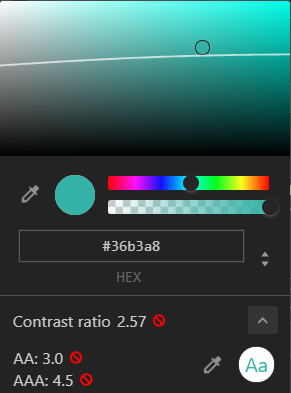
\includegraphics[width=0.3\textwidth]{bjornar/contrast-wcag-aa-small-gronn-tekst.png}}
        \subfigure[blå tekst i logo]{\label{fig:analysis-current-cdt-b}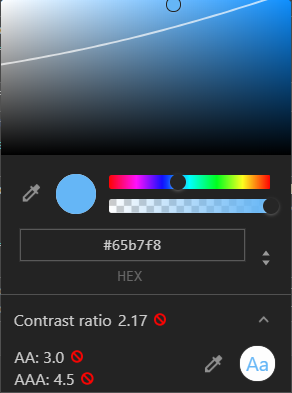
\includegraphics[width=0.3\textwidth]{bjornar/contrast-wcag-aa-small-logo-blaa.png}}
        \subfigure[vanlig tekst]{\label{fig:analysis-current-cdt-c}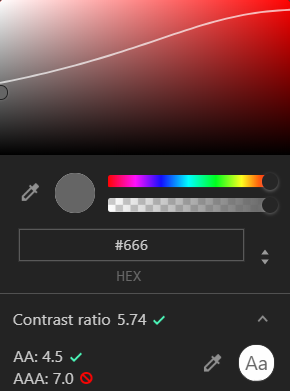
\includegraphics[width=0.3\textwidth]{bjornar/contrast-wcag-aaa-small-body.png}}
        \caption{Google Chrome DevTools - kontrastforhold}
        \label{fig:analysis-current-cdt}
    \end{center}
\end{figure}

Resultatene etter å ha kjørt tester for nivå AAA viser at mesteparten av nettstedet ikke oppfyller kravet for kontrastnivå. Se figur \ref{fig:analysis-current-cca-aaa}. Her blir ingen av avsnittene med ordinær skriftstørrelse markert. Ved å kjøre en test med Chrome DevTools verifiseres påstanden om for dårlig kontrastnivå. Se figur \ref{fig:analysis-current-cdt-c}.

\subsection{WAVE}
Med verktøyet WAVE\footnote{\url{http://wave.webaim.org/}} kan vi videre verifisere funnene som ble gjort i avsnitt \ref{sec:analysis-current-color-contrast-analyzer}. WAVE raporterer om 20 kontrastfeil på nettsiden. \vskip 1em Det ble også oppdaget andre feil:\\ \quad 1x: Dokument språk mangler\\
\quad 4x: Tomme linker\\
\quad 5x: Redudante linker\\
\vskip 1em Annet:\\
\quad 8x: Bilder med tom alt-attributt.\\
\vskip 1em Ved å skru på \q{No-styling} vil man oppdage at det er en skjult seksjon på siden (\q{THE COMPANIES THAT MAKE THEIR LIFE SIMPLE}). Dette blir plukket opp av noen skjermlesere og er derfor ikke ideelt.\\
WAVE viser også at nettstedet har bra stuktur på overskrifter og følger beste praksis.

\subsection{Kontrastforhold mellom tekst og bakgrunnsbilder}
Etter å ha testet kontrasten til siden med verktøyet fra avsnitt \ref{sec:analysis-current-color-contrast-analyzer} og Google Chrome DevTools, vet vi enda ikke om kontrastforholdet i headeren er bra nok. Vi kan se på figur \ref{fig:analysis-current-cca-aa} og \ref{fig:analysis-current-cca-aaa} at det teksten i headeren blir uthevet, og er noe svakere i figur \ref{fig:analysis-current-cca-aaa} enn i \ref{fig:analysis-current-cca-aa}. Dette må vi undersøke nærmere.

Dette er ikke mulig å sjekke med Chrome DevTools eller WAVE. Begge verktøyene vil gi negative resultater som ikke stemmer ettersom de ikke får en bakgrunnsfarge å se på, men et bakgrunnsbilde. Dette fører til at testen ikke blir utført korrekt.

For å løse dette bruker vi Brandwood sin A11y-test\footnote{\url{https://www.brandwood.com/a11y/}}. Verktøyet deler opp bilde i seksjoner og finner gjennomsnittsfargen i hver av disse seksjonene. Deretter sjekkes kontrastforholdet mellom teksten sin farge og fargen i de seksjonene som teksten er over. I figur \ref{fig:analysis-current-a11y_bg-example} kan man se eksempel på resultatet av en test. Her testet vi en hvit tekst mot et bilde av en regnbue. 

\begin{figure}[H]
    \centering
    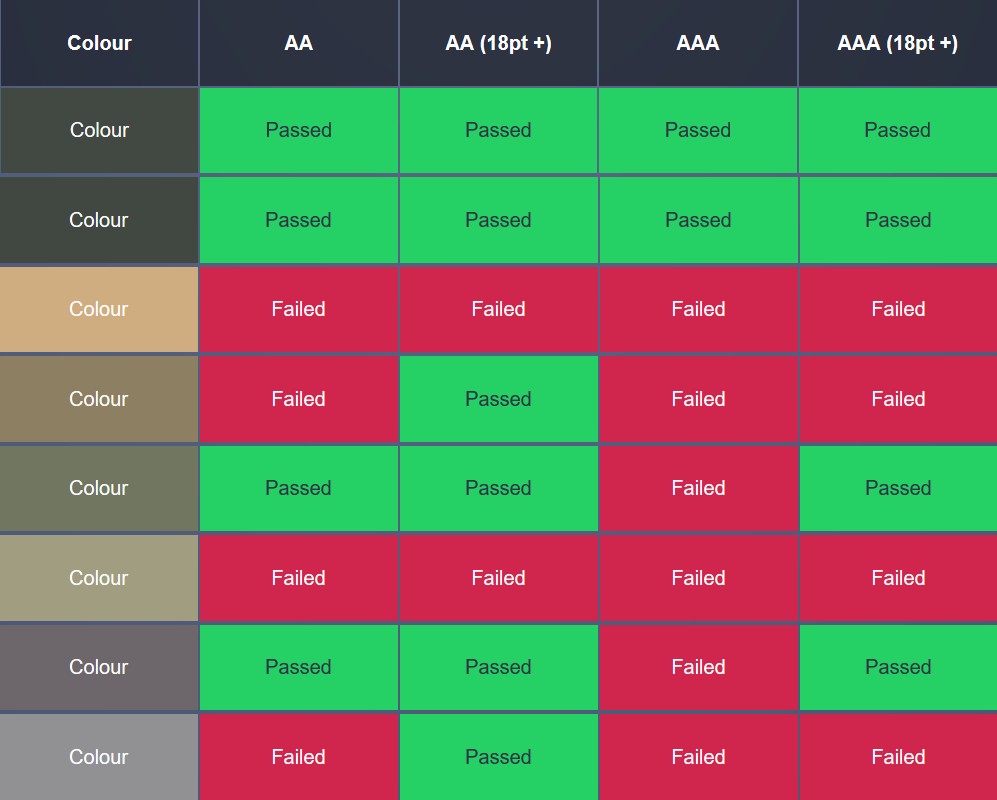
\includegraphics[width=\textwidth]{bjornar/bg-image-eksempel.png}
    \caption{Eksempel}
    \label{fig:analysis-current-a11y_bg-example}
\end{figure}

Vi gjenskapte headeren til Sirkus Media i verktøyet, og testet den store teksten: \q{Vi skaffer konkrete kundehenvendelser} og den mindre teksten \q{Med vår egenutviklede løsning jobber vi for å skaffe våre kunder konkrete kundehenvendelser - direkte på epost og telefon.} Se figur \ref{fig:analysis-current-a11y_bg-generator}. 

\begin{figure}[H]
    \centering
    
\includegraphics[width=\textwidth]{bjornar/bg-image-generator.png}
    \caption{Stor tekst fra header i verktøyet}
    \label{fig:analysis-current-a11y_bg-generator}
\end{figure}

\begin{figure}[H]
    \begin{center}
        \subfigure[Stor tekst]{\label{fig:analysis-current-a11y_bg-h1}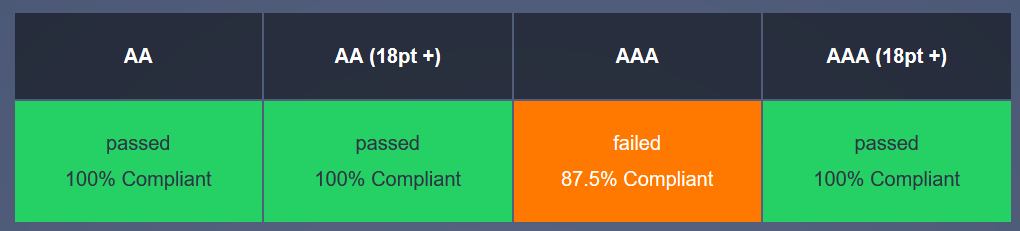
\includegraphics[width=0.475\textwidth]{bjornar/bg-image-h1.png}}
        \subfigure[Liten tekst]{\label{fig:analysis-current-a11y_bg-p}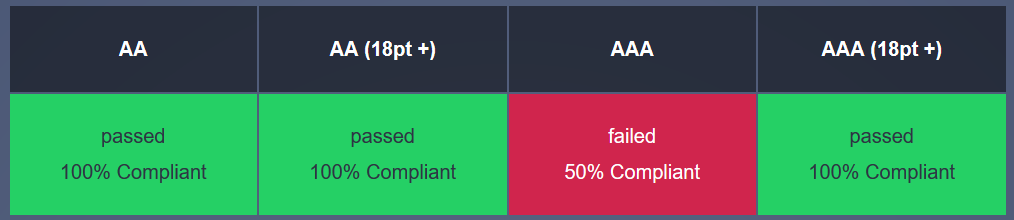
\includegraphics[width=0.475\textwidth]{bjornar/bg-image-p.png}}

        \caption{Testresultat}
        \label{fig:analysis-current-a11y_bg-h1_p}
    \end{center}
\end{figure}

Resultatet som vi ser i figur \ref{fig:analysis-current-a11y_bg-h1_p} viser at teksten i headeren har bra nok kontrastforhold for å passere kravet for AA, men ikke AAA. 

\subsection{Qualys SSL Server Test}
SSL Server Test\footnote{\url{https://www.ssllabs.com/ssltest/}} er en tjeneste som tester SSL og TLS sertifikater. Resultatet på testen ble en A. Dette er bra, men nettstedet burde få et bedre resultatet som A+ eller A++. Det kreves hverken mye tid eller ressurser for å oppnå dette.

\begin{figure}[H]
    \centering
    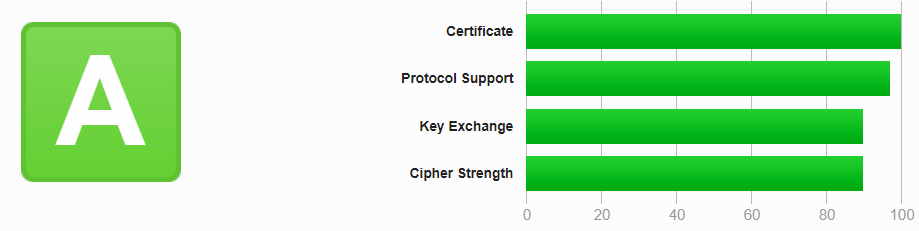
\includegraphics[width=\textwidth]{bjornar/ssllabs.png}
    \caption{Sertifikat score}
    \label{fig:analysis-current-ssl}
\end{figure}

\subsection{Test med skjermleser}
Brukervennligheten via skjermleser ble også testet. Nettsiden ble testet med skjermleseren NVDA\footnote{\url{https://www.nvaccess.org/about-nvda/}}. Det var enkelt å navigere seg rundt på nettsiden. Innholdet kom i en logisk rekkefølge og det var lett å navigere seg mellom elementene. Det eneste problemet var kontaktskjema, som er ganske viktig ettersom målet med nettsiden er at potensielle kunder skal ta kontakt. En annen faktor som manglet var en \q{skip to main content}-link.

\subsection{Google Transparency Report - Safe Browsing: malware and phishing}
Til slutt sjekket vi om nettsiden har skadevare på seg med en tjeneste fra Google\footnote{\url{https://transparencyreport.google.com/safe-browsing/search?url=https://sirkusmedia.no&hl=en-US}}. Her ble det ikke gjort noen funn, noe som selvfølgelig er positivt.

\subsection{Konklusjon}
Ut i fra testene gjort med Google Chrome DevTools, Google Lighthouse og Checkbot kan vi konkludere med at nettsiden er rask. På testen gjort ved høgskolen laster siden inn på under 1 sekund i gjennomsnittet, noe som er meget bra. Siden får over 70\% i poengsum fra Google Lighthouse og Checkbot. Med relativt enkle forbedringer, kan vi få denne summen opp til mellom 90-100\%.

Når det kommer til universell utforming gjør Sirkus Media det bra og følger de lover og regler som gjelder i Norge vedrørende dette. Vi ser likevel at kontrastforholdene på siden er gode nok for kravene til nivå AA, men ikke helt for AAA. Dette er noe som kan forbedres.

Totalt sett gjør nettstedet til Sirkus Media det bra på testene som vi kjørte den gjennom. Som tidligere nevnt er hovedgrunnen til dette at dagens nettsted består av kun en forside og lite informasjon. Dette begrenser muligheten for feil. Det vil være en utfordring å gjøre det like bra i disse testene med et nettsted som består av flere sider, mer innhold og kompleks funksjonalitet.
\clearpage